\documentclass[12pt,a4paper]{scrartcl} %scrartcl berücksichtigt deutsche Formatierungen besser als article
\usepackage[T1]{fontenc}
\usepackage[a4paper, left=3cm, right=2cm, top=2cm, bottom=2cm]{geometry}
\usepackage[activate]{pdfcprot}
\usepackage[ngerman]{babel} %n = neue deutsche Rechtschreibung
\usepackage[parfill]{parskip}
\usepackage[utf8]{inputenc}
\usepackage{kurier}
\usepackage{amsmath}
\usepackage{amssymb}
\usepackage{xcolor}
\usepackage{epstopdf}
%\usepackage{txfonts} % Paket für Word-ähnliche Schriftarten Arial (serifenlos) oder Times New Roman (mit Serifen)
\usepackage{fancyhdr}
\usepackage{graphicx}
\usepackage{prettyref}
\usepackage{hyperref} %Internet-/E-Mail-Verknüpfungen
\usepackage{eurosym}
\usepackage{setspace}
\usepackage{units} % Einheitenpaket
\usepackage{eso-pic,graphicx}
\usepackage{icomma} % nach Komma kein Leerzeichen
\usepackage{textcomp} % fuer spezielle Zeichen, wie \textmu  \textcelsius \textcopyright  \texteuro  \textcent  \textdollar  \textnumero
\usepackage{siunitx}
	%\sisetup{locale = DE,mode = text}         Bruch alles in einer Zeile
	%\sisetup{locale = DE,per-mode = symbol}	  Bruch mit /
	\sisetup{locale = DE,per-mode = fraction} %Bruch als richtiger Bruch
	%im Document:
	%\si{Zahl oder Einheit}
	%\SI{Zahl}{Einheit}		\SI{1,03}{\volt\per\square\metre}
\usepackage{floatrow} % um Bilder mit seitlichem Text zu versehen
%\usepackage[capbesideposition=inside, facing=yes,capbesidesep=quad]{floatrow}


% fuer Grafiken
%\usepackage[pdftex]{color,graphicx}
%\graphicspath{{figures/}}
\DeclareGraphicsExtensions{.png,.jpg,.pdf}
\usepackage{float} % Anwendung: „[H]“ Bild unbedingt an der Stelle, wo \includegraphics steht.
\usepackage{eso-pic,graphicx}
\usepackage{picinpar} % Bilder werden vom Text im folgenden Format umflossen: \begin{window} [#zeilen-vor, position, graphik, titel] Text(der die Grafik umfließen soll) \end{window}

\usepackage{pgfplots} % u.a. für Diagramme
\pgfplotsset{width=14cm,compat=newest}



\definecolor{darkblue}{rgb}{0,0,.5}
\hypersetup{colorlinks=true, breaklinks=false, linkcolor=black, menucolor=black, urlcolor=darkblue} % rote Standardumrandung neu definiert

%\renewcommand{\familydefault}{\sfdefault}  % Textstil serifenlos

\setlength{\columnsep}{2cm}
\newcommand{\fehlt}{\textcolor{red}{Hier fehlen noch Inhalte.}}
\renewcommand{\d}{\, \mathrm d}
\newcommand{\p}{\, \partial}
\newcommand{\dd}[1]{\item[#1] \hfill \\}

\newcommand{\themodul}{Praktikum Optische Technologien}
\newcommand{\thetutor}{Protokoll Versuch polarisiertes Licht}

% Kopf- und Fußzeile
\pagestyle{fancy}
\fancyhead[L]{\footnotesize{M. Nonhoff, C. Hansen, J. Ehlert}}
\chead{\thepage}
\rhead{\footnotesize{\thetutor}}
\lfoot{}
\cfoot{}
\rfoot{}

% Überschriftaufbau
\title{\themodul{}, \\ \thetutor}
\author{Marko Nonhoff, Christoph Hansen, Jannik Ehlert}
\date{} %wenn leer, dann heutiges Datum
\begin{document}

\maketitle
Ort: Laserlabor der Fachhochschule Aachen Campus Jülich
\tableofcontents
\newpage
\vspace{3cm}

\section{Theorie}

In diesem Versuch sollen unterschiedliche Arten von polarisiertem Licht untersucht und bestimmt werden. \\
Um das Gesetz von Malus zu bestätigen, stellen wir im ersten Teil mit dem ersten Polarisator linear polarisiertes Licht her. Dieses betrachten wir mit einer Photodiode durch einen zweiten Polarisator, dessen Filter wir zwischen $\unit[0]{^\circ}$ und $\unit[90]{^\circ}$ variieren. \\
Anschließend stellen wir eine $\lambda/4$ Platte zwischen die beiden Polarisatoren und stellen damit zirkular polarisiertes Licht her. Indem wir nun den zweiten Polarisator zwischen $\unit[-90]{^\circ}$ und $\unit[90]{^\circ}$ variieren, stellen wir fest wie gut unser Licht tatsächlich zirkular polarisiert ist. \\
Im dritten Versuchsteil verdrehen wir die $\lambda/4$ Platte, sodass wir elliptisch polarisiertes Licht erhalten. Hier tragen wir auch wieder die Intensität über $\unit[-90]{^\circ}$ bis $\unit[90]{^\circ}$ auf und leiten daraus ab wie stark elliptisch das Licht polarisiert ist. \\
Im letzten Versuchsteil messen wir mit Hilfe eines Prismas den Brewsterwinkel und bestimmen damit den Brechungsindex des Prismas. Zudem lassen wir einmal p-polarisiertes und einmal s-polarisiertes Licht unter den Winkeln zwischen $\unit[10]{^\circ}$ bis $\unit[80]{^\circ}$ auf das Prisma fallen und messen die Intensität des reflektierten Anteils. Es geht dabei um einen Vergleich mit dem Ergebnis der Fresnel'schen Formeln.


\section{Geräteliste}
\begin{itemize}
\item HeNe Laser
\item Photodiode
\item 2 Polarisatoren
\item Prisma
\end{itemize}


\newpage

\section{Auswertung}

\subsection*{Versuchsteil 1}



\begin{center}
\begin{tabular}{c|c|c|c|c}
	$\theta/^\circ$ & Signal/V & Untergrund/V & bereinigt/V & $\cos^2(\theta)$ \\
	\hline
	&      &      &      &  \\
	0    & 2,002 & 0,009 & 1,993 & 1 \\
	10   & 1,918 & 0,009 & 1,909 & 0,969 \\
	20   & 1,726 & 0,009 & 1,717 & 0,883 \\
	30   & 1,441 & 0,009 & 1,432 & 0,750 \\
	40   & 1,187 & 0,009 & 1,178 & 0,586 \\
	50   & 0,815 & 0,009 & 0,806 & 0,413 \\
	60   & 0,49 & 0,009 & 0,481 & 0,250 \\
	70   & 0,24 & 0,009 & 0,231 & 0,116 \\
	80   & 0,068 & 0,009 & 0,059 & 0,030 \\
	90   & 0,01 & 0,009 & 0,001 & 0,000 \\
\end{tabular}	
\end{center}

In der obigen Tabelle sind unsere Rohdaten, die zum Erstellen des Diagramms verwendet wurde. Man kann den linearen Zusammenhang auch ohne Diagramm direkt sehen, da die Steigung der Geraden nahe bei 2 liegt.



\begin{figure}[H]
	\begin{tikzpicture}
	\begin{axis}[yticklabel style={/pgf/number format/fixed},		
	height=9cm, width=16cm,
	title={Gesetz von Malus},
	legend pos= south east,
	%	     axis x line=middle, % Achse mit Pfeil und Beschriftung am Pfeil
	%	     axis y line=middle,
	xmode=normal,						    % x-Achse 
	ymode=normal,						     % y-Achse 
	xlabel= $\cos^2(\theta)$ ,
	ylabel= Signal/V ,
	grid=both, %major,
		     xmin=-0.1,
		     xmax=1.2,
		     ymin=-0.2,
		     ymax=2.2,
	]
	\addplot[color=blue,only marks,mark=x,mark size=4, error bars/.cd,y dir=both, y explicit] table[x=C,y=B]{Exp_1.txt};
	\addlegendentry{Messwerte};
	\addplot[color=blue,no marks,samples=1000,domain=0:7.5] {1.964*x};
	\addlegendentry{$y = 1,964x$};
	\end{axis} 
	\caption{$I = I_0 \cdot \cos^2(\theta) =\unit[ 2,002]{mV} \cdot \cos^2(\theta)$}
	\end{tikzpicture}
\end{figure}

Wenn wir uns das Diagramm betrachten, stellen wir fest, das der lineare Zusammenhang sehr gut getroffen wird. Die leichten Schwankungen der Punkte um die Linie führen wir auf den variierende Laserleistung zurück. 



\newpage


\subsection*{Versuchsteil 2}

Hier ging es darum möglichst gut zirkular polarisiertes Licht herzustellen. In einem Diagramm haben wir das gemessene Ausgangssignal über den Winkel des zweiten Polarisators aufgetragen. Dabei sollten der Theorie nach alle Punkte auf einer Parallelen zur x-Achse liegen.


\begin{figure}[H]
	\begin{tikzpicture}
	\begin{axis}[yticklabel style={/pgf/number format/fixed},		
	height=9cm, width=16cm,
	title={zirkular polarisiertes Licht},
	legend pos= south east,
	%	     axis x line=middle, % Achse mit Pfeil und Beschriftung am Pfeil
	%	     axis y line=middle,
	xmode=normal,						    % x-Achse 
	ymode=normal,						     % y-Achse 
	xlabel= $\theta/^\circ$ ,
	ylabel= Signal/V ,
	grid=both, %major,
	xmin=-90,
	xmax=90,
	ymin=0,
	ymax=1.1,
	]
	\addplot[color=blue,only marks,mark=x,mark size=4, error bars/.cd,y dir=both, y explicit] table[x=W,y=B]{Exp_2.txt};
	\addlegendentry{Messwerte};
	\addplot[color=blue,no marks,samples=1000,domain=-90:90] {0.93};
	\addlegendentry{$y = 0,93$};
	\end{axis} 
	\end{tikzpicture}
\end{figure}


\newpage


Wenn wir die Rohdaten betrachten, stellen wir fest, das wir eine Schwankungsbreite von $\approx \unit[70]{mV}$ haben. 

\hfill \\

\begin{center}
\begin{tabular}{c|c|c|c}
	$\theta/^\circ$ & Signal/V & Untergrund/V & bereinigt/V \\
	\hline
	&      &      &  \\
	-90  & 0,921 & 0,007 & 0,914 \\
	-80  & 0,918 & 0,007 & 0,911 \\
	-70  & 0,919 & 0,007 & 0,912 \\
	-60  & 0,926 & 0,007 & 0,919 \\
	-50  & 0,939 & 0,007 & 0,932 \\
	-40  & 0,941 & 0,007 & 0,934 \\
	-30  & 0,93 & 0,007 & 0,923 \\
	-20  & 0,925 & 0,007 & 0,918 \\
	-10  & 0,954 & 0,007 & 0,947 \\
	0    & 0,951 & 0,007 & 0,944 \\
	10   & 0,951 & 0,007 & 0,944 \\
	20   & 0,975 & 0,007 & 0,968 \\
	30   & 0,974 & 0,007 & 0,967 \\
	40   & 0,965 & 0,007 & 0,958 \\
	50   & 0,936 & 0,007 & 0,929 \\
	60   & 0,927 & 0,007 & 0,92 \\
	70   & 0,925 & 0,007 & 0,918 \\
	80   & 0,907 & 0,007 & 0,9 \\
	90   & 0,904 & 0,007 & 0,897 \\
\end{tabular}	
\end{center}

\hfill \\


Wir erachten dieses Ergebnis als gut, da die Schwankungsbreite nur $ \approx \unit[7]{\%}$ des Signals beträgt. Für noch besser zirkular polarisiertes Licht müsste man noch mehr Zeit in die Kallibration der Apparatur stecken, aber das würde leicht die zeitlichen Grenzen des Praktikums und der Studenten sprengen.


\newpage


\subsection*{Versuchsteil 3}

Wir haben die $\lambda/4$ Platte aus dem zweiten Versuchsteil verdreht um elliptisch polarisiertes Licht zu erhalten. Anschließend haben wir wieder von $\unit[-90]{^\circ}$ bis $\unit[90]{^\circ}$ die Intensität gemessen:

\hfill \\

\begin{center}
\begin{tabular}{c|c|c|c}
	Winkel & Signal & Untergrund & bereinigt \\
	\hline
	&      &      &  \\
	-90  & 0,513 & 0,007 & 0,506 \\
	-80  & 0,374 & 0,007 & 0,367 \\
	-70  & 0,305 & 0,007 & 0,298 \\
	-60  & 0,318 & 0,007 & 0,311 \\
	-50  & 0,409 & 0,007 & 0,402 \\
	-40  & 0,565 & 0,007 & 0,558 \\
	-30  & 0,759 & 0,007 & 0,752 \\
	-20  & 0,985 & 0,007 & 0,978 \\
	-10  & 1,234 & 0,007 & 1,227 \\
	0    & 1,43 & 0,009 & 1,421 \\
	10   & 1,571 & 0,007 & 1,564 \\
	20   & 1,685 & 0,009 & 1,676 \\
	30   & 1,686 & 0,009 & 1,677 \\
	40   & 1,592 & 0,009 & 1,583 \\
	50   & 1,393 & 0,009 & 1,384 \\
	60   & 1,192 & 0,009 & 1,183 \\
	70   & 0,961 & 0,009 & 0,952 \\
	80   & 0,722 & 0,009 & 0,713 \\
	90   & 0,513 & 0,008 & 0,505 \\
\end{tabular}	
\end{center}

\hfill \\

Aus den Intensitäten, die wir bei $\unit[0]{^\circ}$ und bei $\unit[90]{^\circ}$ gemessen haben, können wir nun den Winkel $\phi$ berechnen, der die Ellipsizität quantifiziert.

\begin{align*}
\tan^2(\phi) &= \frac{I(0)}{I(90)} \\
\Leftrightarrow \phi = \arctan\left( \sqrt{\frac{I(0)}{I(90)}} \right) &= \arctan\left( \sqrt{\frac{I(1,421)}{I(0,506)}} \right) = \unit[59,16]{^\circ}
\end{align*}


\newpage



Graphisch sieht das ganze dann so aus:


\begin{figure}[H]
	\begin{tikzpicture}
	\begin{axis}[yticklabel style={/pgf/number format/fixed},		
	height=9cm, width=16cm,
	title={zirkular polarisiertes Licht},
	legend pos= south east,
	%	     axis x line=middle, % Achse mit Pfeil und Beschriftung am Pfeil
	%	     axis y line=middle,
	xmode=normal,						    % x-Achse 
	ymode=normal,						     % y-Achse 
	xlabel= $\theta/^\circ$ ,
	ylabel= Signal/V ,
	grid=both, %major,
	xmin=-90,
	xmax=90,
	ymin=0,
	ymax=1.8,
	]
	\addplot[color=blue,only marks,mark=x,mark size=4, error bars/.cd,y dir=both, y explicit] table[x=W,y=B]{Exp_3.txt};
	\addlegendentry{Messwerte};
	\end{axis} 
	\end{tikzpicture}
\end{figure}


Nun können wir noch das Verhältnis des ordentlichen ($E_1$) und des außerordentlichen ($E_2$) Feldvektors berechnen:

\begin{align*}
E_1 &= E(t) \cdot \sin(\theta) = E(t) \cdot 0,85 \\
E_2 &= E(t) \cdot \cos(\theta) = E(t) \cdot 0,51 \\
\Rightarrow \frac{E_1}{E_2} &= 1,67
\end{align*}


\newpage


\subsection*{Versuchsteil 4}

Wir haben nun mit einem Prisma einmal den s-polarisierten Teil des Lichts und einmal den p-polarisierten Teil des Lichtes betrachtet. 


%\begin{figure}[H]
%	\begin{tikzpicture}
% 	height=9cm, width=16cm,
%	title={Reflexion am Prisma},
%	legend pos= north west,
	%	     axis x line=middle, % Achse mit Pfeil und Beschriftung am Pfeil
	%	     axis y line=middle,
%	xmode=normal,						    % x-Achse 
%	ymode=normal,						     % y-Achse 
%	xlabel= $\theta/^\circ$ ,
%	ylabel= Signal/V ,
%	grid=both, %major,
%	xmin=0,
%	xmax=90,
%	ymin=0,
%	ymax=0.7,
%	\addplot[color=red,only marks,mark=x,mark size=4, error bars/.cd,y dir=both, y explicit] table[x=W,y=I]{Exp_4_p-pol.txt};
%	\addplot[color=blue,only marks,mark=+,mark size=4, error bars/.cd,y dir=both, y explicit] table[x=W,y=I]{Exp_4_s-pol.txt};
%	\addlegendentry{p-polarisiert};
%	\addlegendentry{s-polarisiert};
%	\addplot[color=green,no marks,samples=1000,domain=0:85] {0.026*exp(0.0355*x)};
%	\addplot[color=green,no marks,samples=1000,domain=0:85] {2*10^(-9)*x^5 - 3*10^(-7)*x^4 + 2*10^(-5)*x^3 - 0.0008*x^2 + 0.0115*x - 0.0176};
%	\end{axis} 
%	\end{tikzpicture}
%\end{figure}


\begin{figure}[h]
	\centering
	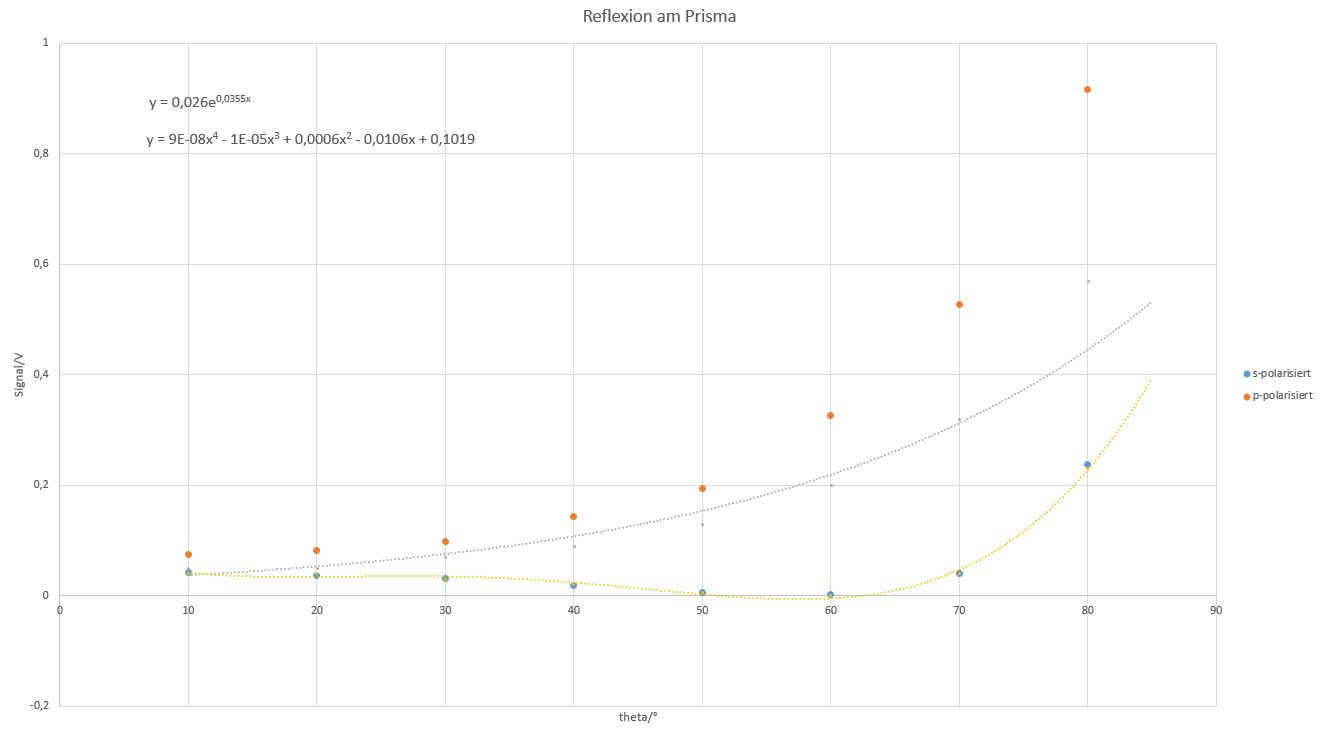
\includegraphics[scale=0.5]{Graphik_Teil_4.jpg}
\end{figure}




Wir sehen anhand des Graphen für p-polarisiertes Licht, das der Brewsterwinkel in der Nähe von $\unit[60]{^\circ}$ liegen muss. Bei genauerem messen, stellten wir fest, das der Brewsterwinkel bei unserem Prisma $\unit[57,75]{^\circ}$ ist. Das entspricht einem Brechungsindex von 1,58.

Den Winkel $\beta$ haben wir nach der Formel in der Anleitung berechnet und kamen dabei auf folgende Werte für die Reflexionsgrade:

\hfill

\begin{center}
	\begin{tabular}{c|c|c|c}
		$\alpha$ & $\beta$ & $R_S$   & $R_P$ \\
		\hline
		&       &       &  \\
		10    & 6,31  & 0,05  & 0,04 \\
		20    & 12,5  & 0,05  & 0,04 \\
		30    & 18,45 & 0,07  & 0,03 \\
		40    & 24,01 & 0,09  & 0,02 \\
		50    & 29    & 0,13  & 0,005 \\
		60    & 33,24 & 0,2   & 0,0008 \\
		70    & 36,48 & 0,32  & 0,04 \\
		80    & 38,56 & 0,57  & 0,23 \\
	\end{tabular}
\end{center}

\hfill

Wie wir auf der Graphik sehen passen unsere Messungen des p-polarisierten Lichts sehr gut zum idealen Verlauf. Allerdings ist die gemessene Reflexionsrate bei s-polarisertem Licht sehr viel größer als man anhand des idealen Verlaufes vermuten würde. Warum das so ist, können wir uns nicht erklären.



\section{Fehlerbetrachtung}

Im Versuchsteil 2 ist die einstellbare $\lambda/4$ Platte der Hauptfehlergrund. Man kann diese Konstruktionsbedingt nur auf ca $\unit[1-2]{^\circ}$ genau einstellen, daher erhalten wir auch keine hundertprozentige Parallele. \\
Zudem kennen wir den systematischen Fehler des Transmissionsdetektors und des Anzeigegerätes nicht.






























\end{document}
